\section{Evaluation}
\label{sec:Evaluation}
We collected data from $9$ subjects, each using our instrumented visualization for approximately $50$ minutes on a series of structured and unstructured tasks. We used the collected data to test the validity and effectiveness of collecting eye-tracking data in visualization space in two ways. 
First, we quantitatively compare the results produced by our automatic instrumentation, to annotations produced by human coders. Specifically, we compared the similarity of our results to human annotations, with the similarity between human annotations. We found that our results are on average as similar to human annotations as are human annotations similar to each other. Moreover, we conducted this analysis for all three viewed detection algorithms described in sections~\ref{sec:AOIBasedViewedObjectDetection} and~\ref{sec:MehthodsIntelligentAlgorithm} and showed that the AOI based method described in section~\ref{sec:AOIBasedViewedObjectDetection} performs poorly compared to the other two, and that the prediction component described in section~\ref{sec:MehthodsIntelligentAlgorithm} improves detection accuracy by about $5\%$  (Figure~\ref{sayeed}). Second, we show that our instrumentation method can provide useful information by providing evidence that viewed objects detected by our instrumentation align with the tasks we asked people to do.

\subsection{Study Design }

\textbf{Setup: } We used the visualization and data described in section~ref{Sayeed}, and a lightweight $60$Hz EyeX eye-tracker from Tobii connected to a 17'' monitor. Subjects were seated approximately $30''$ away from the display. 

\textbf{Subjects:} We collected data from $9$ graduate and undergraduate students with ages ranging between $20$ years and $30$ years. Six of them were male and three were female. Subjects were paid $10$ for their participation. 

\textbf{Protocol:} Subjects were first given a description of the study's purpose and protocol. They were then introduced to our IMDB PivotPaths visualization and asked to perform a few training tasks to help them get accustomed with the visualization. This introductory part lasted approximately $10$ minutes on average. The main section of the study followed, involved multiple instances of four types of tasks, and lasted approximately $50$ minutes. 


\textbf{Tasks:} We asked subjects to complete four types of tasks. We aimed to balance structured tasks and unstructured tasks. To solve the structured tasks, subjects had to consider a set of objects that was better defined and less variable than in unstructured tasks. This made it easier for us to test the degree to which our detection of viewed objects is aligned with the data required to complete the tasks. On the other hand, data collected for unstructured tasks may be better at informing designs of future analysis systems of such data. We limited the time we allowed subjects to spend on each task. This was done for two reasons: to limit the total duration of the study, and to make results comparable across time and users.

\begin{itemize}
	\item \textbf{Task1 (structured):} Finding four commonalities between pairs of movies. The tasks were limited at three minutes each, and subjects solved the following four instances of this task: (i) Raiders of the Lost Ark and Indiana Jones and the Last Crusade; (ii) A and B; (iii) C and D; (iv) E and F.  
	\item \textbf{Task2 (structured):} Ranking collaborations between a director and three actors ($2$ minutes).  Subjects complete the following four task instances: A and B,C,D; 
	\item \textbf{Task4 (semi-structured):} Given three movies, subjects were asked to recommend a fourth ($5$ minutes). Subjects solved three such tasks: 
	\item \textbf{Task5 (unstructured):} Given a brief and incomplete description of the ``Brat Pack'', a group of young actors popular in the 80's, subjects were asked to find additional members and movies they acted in. Subjects solved one such task, in approximately $5$ minutes. 
\end{itemize}

\subsection{Result: data collected automatically is similar to that of human annotators}
\label{sec:EvalResults}

We compared lists of viewed objects produced by our instrumentation to similar lists created manually by human coders who visually inspected screen shots together with gaze positions. To this end, we enlisted the help of four coders and asked them to code data corresponding to one task of approximately three minutes, for six subjects. The six subjects were selected randomly and were the same for all four coders. 

Coders were asked to indicate what they thought the subjects looked at, and note the start and end time of each object's viewing, at a resolution of $100$ms. They were allowed to indicate multiple objects if they were unsure which of those objects was viewed. Coders used an application that allowed them to look at screen shots and of the users� activity with overlayed gaze positions. They  advanced through the data in $100$ms increments, and annotated it as requested. Each coder spent approximately one hour on each of the six subjects.

We transformed the data provided by each coder for each user into a long vector with a position for each $100$ms that was analyzed, and their coding result for that particular $100$ms interval. We then created a similar representation from our automatically collected data. We defined a similarity measure between two such vectors as the percentage of temporally aligned cells from the two vectors that are equal. Equality between cells was defined as a non-empty intersection between their contents. Finally, we computed such similarities between each coder and the automatically generated annotation for each of the two users ($4$ coders $\times$ $2$ subjects $\times$ $1$ automated annotation $=$ $8$ similarities), and similarities between all pairs of coders for each subject ($6$ coder pairs $\times$ $2$ subjects $=$ $12$ similarities). These similarities are shown in Figure~\ref{fig:quantitative}. As can be seen, the similarities between the results of human coders and our instrumentation are very close to the similarities between coders. 

The data we collected allowed us to do this analysis for all three approaches 3.1-3.3. Specifically, if we only consider gaze scores $gs$ equal to one, we essentially have the output of the AOI approach described in section 1. If we limit the analysis to $gs$ scores alone, without the prediction component described in 3.3, we have the output of the probabilistic approach described in section 3.2 .

\textbf{Validity of evaluation:} Our evaluation should be seen primarily as one that tests the ability of our algorithm to outperform the state of the art as captured by human coders, rather than one that validates our algorithm against a ground truth. Specifically, it doesn�t test how close our method can get to a ground-truth, but instead shows that our method can provide data of quality similar to the state of the art analysis method, human coders, with significant less effort and much faster. This distinction is important because there is a question as to whether human coders can provide an accurate ground-truth against which to evaluate our methods. We think that the notion of a ground-truth in this application is slightly misguided and discuss this aspect in our discussion section. 

\begin{figure}[htb]
  \centering
  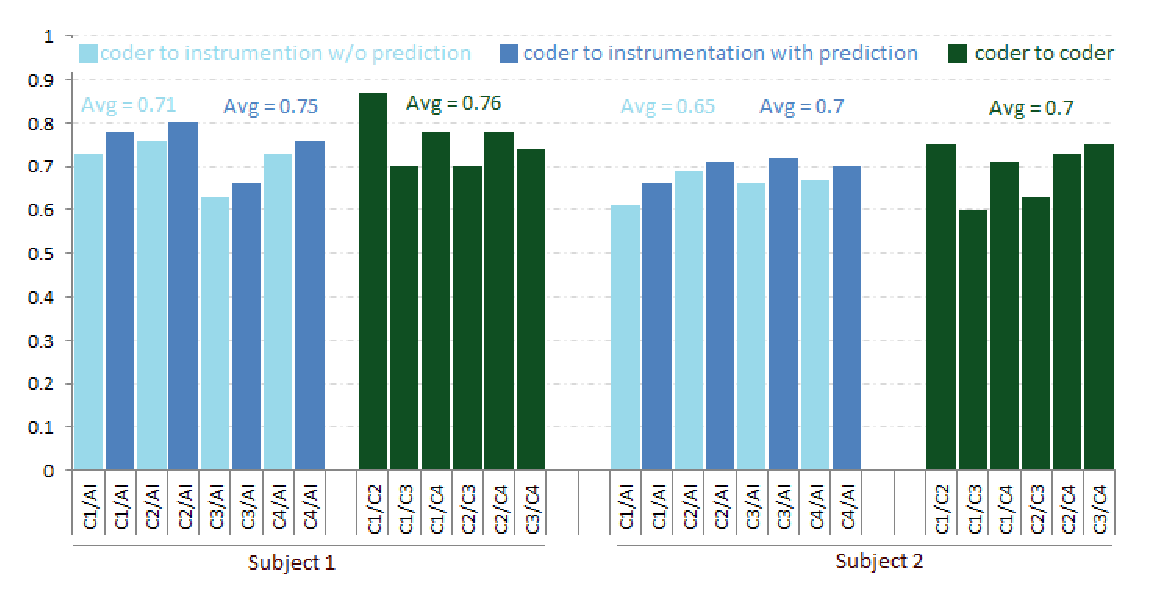
\includegraphics[width=\linewidth]{images/quantitative.eps}
  \caption{Similarities of viewing scores computed with viewed object prediction (dark blue), and without prediction (light blue) to annotations by four human coders (C1-4), are compared to similarities between the human coders own results (green), for two subjects. }
	\label{fig:quantitative}
\end{figure}

\subsection{Results: data collected automatically is relevant and useful}
We show object viewing activity over time using a heatmap representation, by discretizing time and displaying it horizontally, and listing viewed objects vertically. The viewed objects listed vertically were colored based on their type (movie, actor, director, genre) and could be sorted based on either first time they were viewed, amount of viewing activity, or type. 
Showing viewing data at multiple time scales requires a method of aggregating viewing scores collected every $15$ms into larger time intervals. While it may be interesting to explore the effects of different aggregation strategies, our current system only implemented one. We use Formula~\ref{eq:Aggregate} to compute the aggregated score of $O_i$ in time interval $T$. Intuitively, the formula averages all non-zero viewing scores collected in interval $T$, but also takes into account the duration of $T$. For instance, six high viewing scores recorded in a $100$ms time span are sufficient to yield a high aggregated score for that interval ( $\frac{100 \times 60 }{1000} = 6$), while for a $1000$ms interval we would require $60$ high viewing scores ( $\frac{1000 \times 60 }{1000} = 60$).
\begin{equation}
aggScore(T,O_i) = \frac{\displaystyle\sum_{t \in T }{vs(t, O_i)}}{\max (count(vs(t, O_i) > 0 , t \in T),|T| \times \frac{60}{1000}) }
\label{eq:Aggregate}
\end{equation}

The top of Figure~\ref{fig:heatmap} shows data for the first four tasks aggregated over all ten users. The four clusters noticeable in the heatmap provide a first indication that elements viewed by users are in tight correlation with the four tasks they had to do, which is in accordance with our hypothesis and expectation. However, the four different clusters appearing in the heatmap are not sufficiently telling, since the views involved in each task were distinct and showed different data. As such, even a random sampling of objects from these views could produce a similar high level clustering in the heatmap. 

\begin{figure*}[htb]
  \centering
  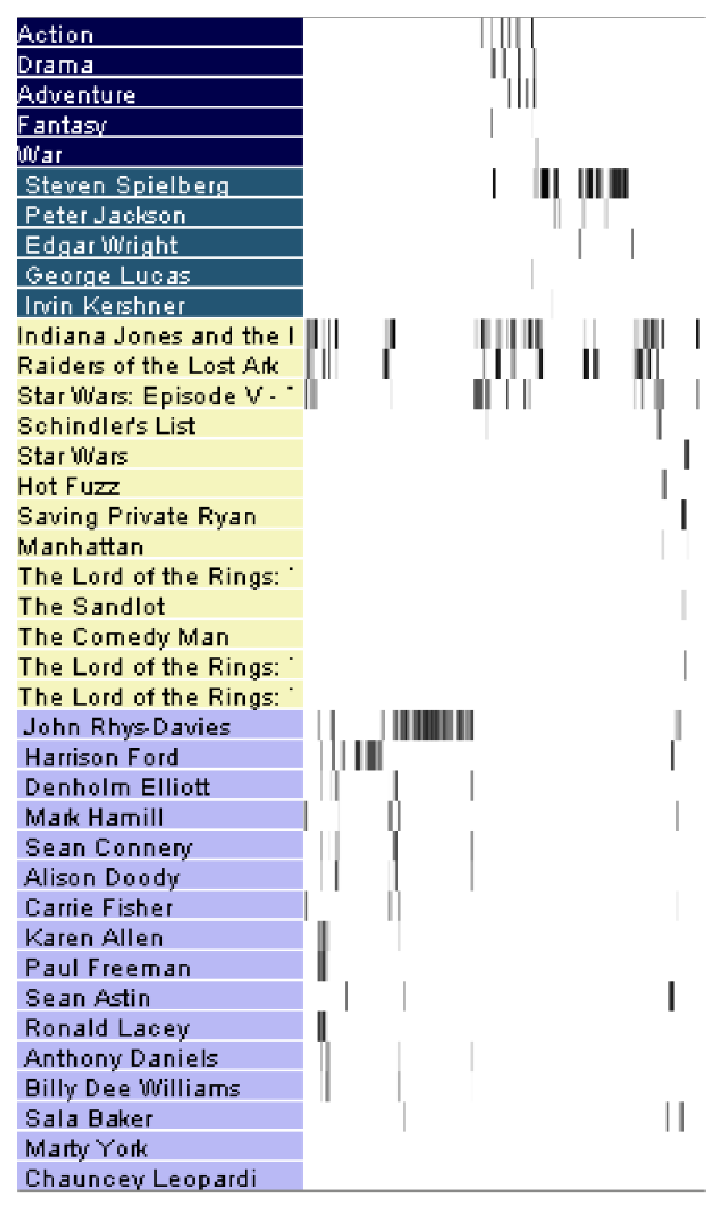
\includegraphics[width=\linewidth]{images/heatmap.eps}
  \caption{(Top) Aggregated data for all ten users reveals three clusters of viewed objects corresponding to the first three tasks that subjects were asked to do. (Middle) Sorting the heatmap by how much each object was viewed shows, as hypothesized, that objects most relevant to the task, finding commonalities between Raiders of the Lost Ark and Indiana Jones and the Last Crusade, were viewed most often. (Bottom) Sorting the heatmap by which objects were viewed first, reveals interesting temporal patterns for a particular user. }
	\label{fig:heatmap}
\end{figure*}

A closer look at the specific data objects listed in the heatmap, as well as their associated viewing activity, removes this concern. In Figure~\ref{fig:heatmap} middle, we restricted the heatmap to showing only data corresponding to the second task subjects completed, which was finding the similarities between the movies ``Raiders of the Lost Ark'' and ``Indiana Jones and the Last Crusade''. The view involved in solving this task contained about $70$ actors, $16$ movies, $11$ directors, and $15$ genres, yet the heatmap reveals that only a small subset of these elements were viewed regularly, and that the more connected the data element was to the task, the more often and intently it was viewed.

Moreover, looking at the data for a single user, sorted by first view, (Figure~\ref{fig:heatmap}) bottom, reveals temporal patterns in how the subject solved the task: they looked at movie titles throughout the task, though predominantly in the beginning, actors in the first half, in a fairly consistent sweep, and directors and genres in the second half. 

\textbf{Validity of evaluation:} This type of evaluation comes closer to the notion of a ground-truth evaluation. The tasks, especially the structured ones, dictate what users will have to look at in order to solve the tasks, and thus suggest an approximate ground-truth. 

Moreover, the fact that the data we collected is tightly correlated suggests and the analyses we were able to perform on it suggest that the data is useful. In a real life analysis using such instrumentation, evaluators would not necessarily know what the tasks are but our evaluation shows that they could determine what users are trying to do because their data would be correlated with the tasks. We also showed that particular strategies and insights were possible from the data alone. 
